\chapter{Extensiones al Programa Original}
\label{cap:extensiones}

Una vez comentadas las motivaciones, objetivos y planteamiento de trabajo, se tratarán los puntos en los que se ha trabajado para lograr la realización del proyecto. En este capítulo se incide en las extensiones y cambios realizados, tratados a bajo nivel y desde un punto de vista técnico.

\section{Adaptación para la ejecución de comandos desde la interfaz}

Como se ha comentado en varias ocasiones, siguiendo el objetivo principal de democratizar el uso de esta herramienta para perfiles no tecnológicos como psicólogos u otros profesionales, uno de los desafíos era hacer la aplicación disponible únicamente desde la interfaz, de modo que los usuarios interactúen con la interfaz para realizar todas las acciones.

Originalmente, si los usuarios querían elegir una simulación, ejecutarla o guardarla, por ejemplo, debían ejecutar estas acciones desde la terminal. Esto podría ser una barrera de entrada para ciertos usuarios que no estén familiarizados con estas tecnologías. El objetivo era hacerla accesible desde la interfaz únicamente.

Para conseguirlo, se plantearon ciertas opciones. Tras investigarlas, se tomó la decisión de optar por la opción representada en el diagrama de la figura \ref{fig:DiagramaComandos}, ya que no implicaría cambiar la arquitectura actual de la aplicación, en la cual son los comandos ejecutados en la terminal del backend los que indican las acciones a realizar y marcan las llamadas al modelo de lenguaje.

\begin{figure}[h]
	\centering
	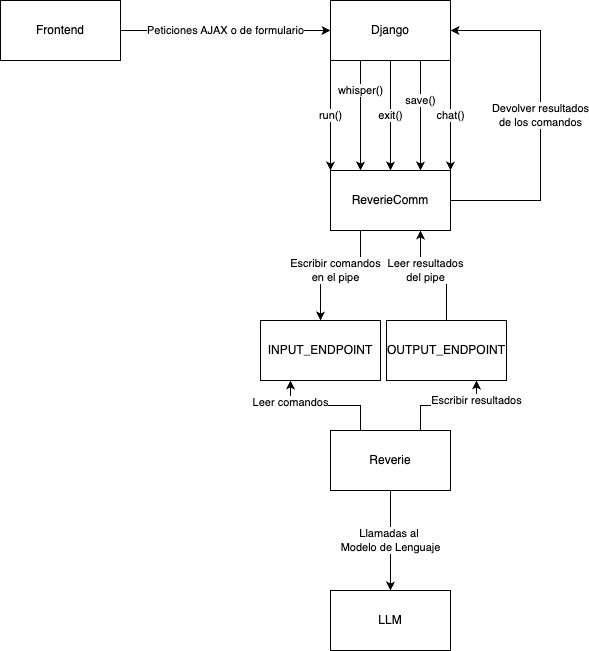
\includegraphics[width = 0.6\textwidth]{Imagenes/Vectorial/DiagramaComandos.png}
	\caption{Diagrama del estado de los comandos actualmente}
	\label{fig:DiagramaComandos}
\end{figure}

Como se aprecia en el diagrama, realmente siguen existiendo las llamadas de los comandos, pero se redirecciona para que se ejecuten desde la interacción con la interfaz. 

El flujo siempre comienza desde la propia interfaz, el front end. Mediante esta se hacen peticiones a django, que es el primero de los back ends, el que se encarga de cargar los datos, redirigir las vistas y comunicarse con el segundo de los backends (el que hemos llamado Reverie en el diagrama). Tras las llamadas a django, este se comunicará con una nueva clase, conocida como ReverieComm, para ejecutar los comandos mediante el uso de pipes. En una pipe habrá un fichero FIFO en el que se escribirán los comandos que deben de ser ejecutados, y el backend Reverie los leerá y ejecutará en orden, escribiendo la respuesta del modelo de lenguaje en otro fichero, para que sea leído por la clase ReverieComm y transmitido a Django, para que finalmente sea mostrado por pantalla mediante el front end.

De esta manera, logramos solucionar el problema de que los usuarios tengan que interactuar directamente con la terminal y al mismo tiempo no modificamos la arquitectura, ya que los comandos seguirán siendo ejecutados. 

\section{Interacción total con el sistema mediante la interfaz gráfica}

\textcolor{red}{POR HACER}

\section{Funcionalidad de chat con los agentes en tiempo real}

\textcolor{red}{POR HACER}

\section{Funcionalidad de resúmenes de las simulaciones}

\textcolor{red}{POR HACER}

